% !TeX spellcheck = cs_CZ
{\tikzset{external/prefix={tikz/FYZII/}}
 \tikzset{external/figure name/.add={ch27_}{}}
%---------------------------------------------------------------------------------------------------
% file fey2ch27.tex
%---------------------------------------------------------------------------------------------------
%=========================== Kapitola Energie pole a hybnost pole ==================================
\chapter{Energie pole a hybnost pole}\label{fyz:IIchaXXVII}
\minitoc
  \section{Lokální zákony zachování}\label{fyz:IIchaXXVIIsecI}
  \section{Zákon zachování energie a elektromagnetizmus}\label{fyz:IIchaXXVIIsecII}
  \section{Hustota energie a hustota toku energie elektromagnetického 
  pole}\label{fyz:IIchaXXVIIsecIII}
  \section{Nejednoznačnost energie pole}\label{fyz:IIchaXXVIIsecIV}
  \section{Příklady hustoty toku energie}\label{fyz:IIchaXXVIIsecV}
  \section{Hybnost pole}\label{fyz:IIchaXXVIIsecVI}
  \section{Příklady a cvičení}\label{fyz:IIchaXXVIIsecVII}

    \begin{figure}[ht!] %\ref{fyz_fig609}
      \centering
      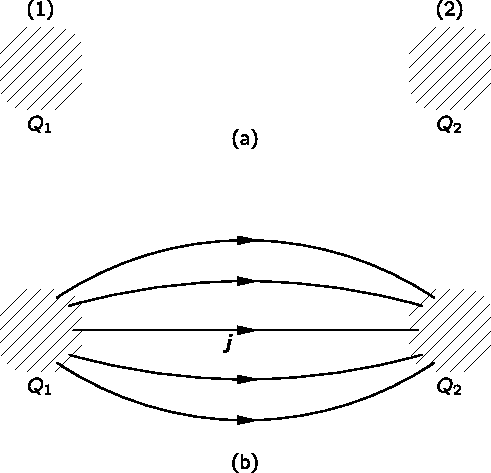
\includegraphics[width=0.7\linewidth]{fyz_fig609.pdf}
      \caption{
               (\cite[s.~707]{Feynman02})}
      \label{fyz_fig609}
    \end{figure}

    \begin{figure}[ht!] %\ref{fyz_fig610}
      \centering
      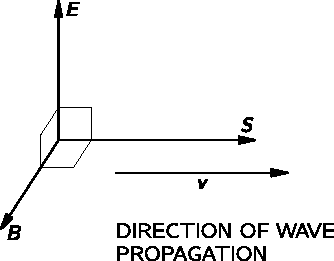
\includegraphics[width=0.7\linewidth]{fyz_fig610.pdf}
      \caption{
               (\cite[s.~707]{Feynman02})}
      \label{fyz_fig610}
    \end{figure}

    \begin{figure}[ht!] %\ref{fyz_fig611}
      \centering
      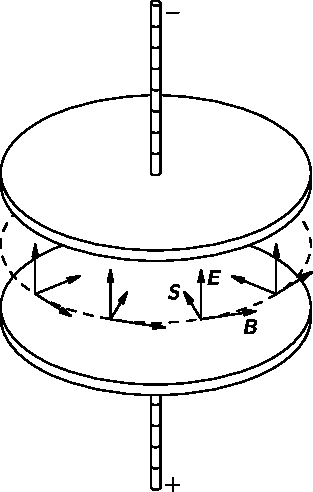
\includegraphics[width=0.7\linewidth]{fyz_fig611.pdf}
      \caption{
               (\cite[s.~707]{Feynman02})}
      \label{fyz_fig611}
    \end{figure}

    \begin{figure}[ht!] %\ref{fyz_fig612}
      \centering
      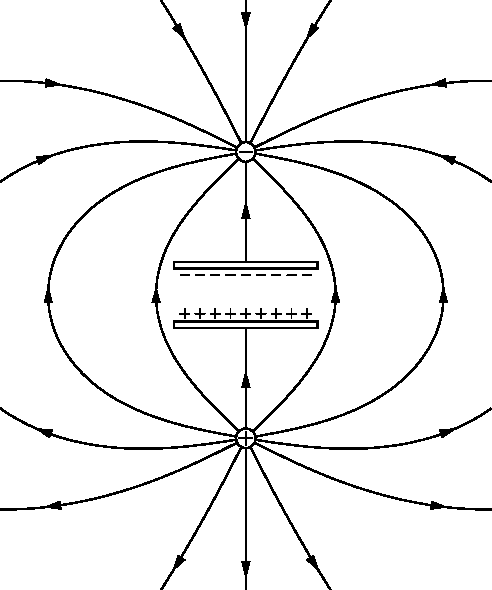
\includegraphics[width=0.7\linewidth]{fyz_fig612.pdf}
      \caption{
               (\cite[s.~707]{Feynman02})}
      \label{fyz_fig612}
    \end{figure}

    \begin{figure}[ht!] %\ref{fyz_fig613}
      \centering
      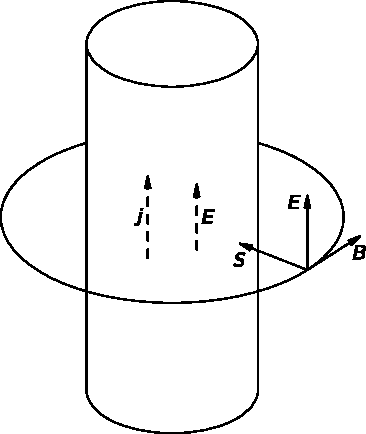
\includegraphics[width=0.7\linewidth]{fyz_fig613.pdf}
      \caption{
               (\cite[s.~707]{Feynman02})}
      \label{fyz_fig613}
    \end{figure}

    \begin{figure}[ht!] %\ref{fyz_fig614}
      \centering
      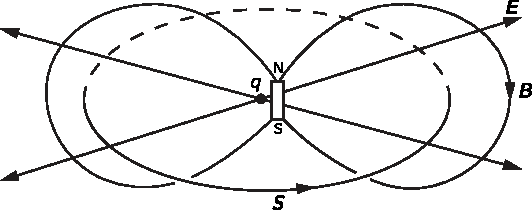
\includegraphics[width=0.7\linewidth]{fyz_fig614.pdf}
      \caption{
               (\cite[s.~707]{Feynman02})}
      \label{fyz_fig614}
    \end{figure}

    \begin{figure}[ht!] %\ref{fyz_fig615}
      \centering
      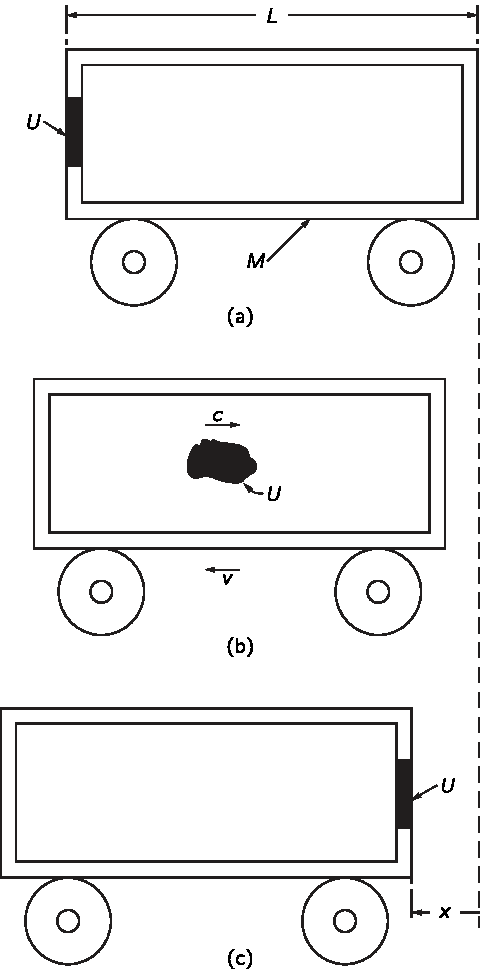
\includegraphics[width=0.7\linewidth]{fyz_fig615.pdf}
      \caption{
               (\cite[s.~707]{Feynman02})}
      \label{fyz_fig615}
    \end{figure}

    \begin{figure}[ht!] %\ref{fyz_fig616}
      \centering
      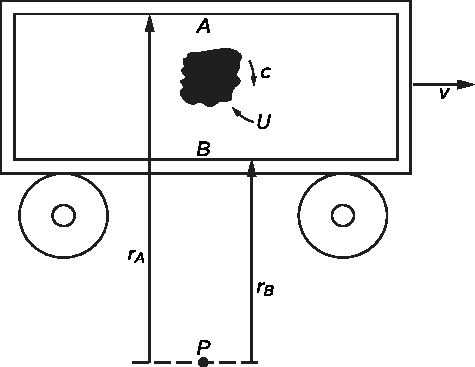
\includegraphics[width=0.7\linewidth]{fyz_fig616.pdf}
      \caption{
               (\cite[s.~707]{Feynman02})}
      \label{fyz_fig616}
    \end{figure}

} %tikzset
%---------------------------------------------------------------------------------------------------
\printbibliography[title={Seznam literatury},heading=subbibliography]
\addcontentsline{toc}{section}{Seznam literatury}